\section{Evaluation}
\label{sec:evaluation}

We evaluate the costs of reusing resident kernel implementations, from
individual mappings and dependency bindings to complete algorithms and
a continuously updated subsystem. Section~\ref{sec:page-grafting}
separates execution through established mappings from mapping faults
and backing-page read-in. Section~\ref{sec:dependency-overhead} examines
existing and newly introduced indirection, followed by complete kernel
routines. Section~\ref{sec:exported-algorithms} uses intermediate
implementations to distinguish source adaptation, build context, and
dependency selection in actual exports.
Section~\ref{sec:clocktime} evaluates how a shared time-reading
implementation changes code organization, state publication, and query
cost, and then measures its application-level effect in Nginx.
Section~\ref{sec:filesystem-reuse} extends the evaluation to filesystem
code with domain-private objects, real container execution, and common-core
maintenance.

All experiments use an Intel Core i7-1165G7 with four physical cores,
SMT disabled, and GCC~11.4.0. Microbenchmarks and Clocktime user readers
run on CPU~2; the Clocktime controller runs on CPU~0. Page-grafting,
PGOT, and algorithm experiments use Linux 5.15.0-119-generic; Clocktime
uses custom Linux 5.15.198 kernels, as do the filesystem hardware measurements.
PGOT compares builds with and without
inline retpolines. Clocktime READ and UPDATE compare Raw and VKSO within
each of two fixed mitigation configurations, Normal and no-retpoline;
the Nginx experiment uses Normal.

Isolated execution timings exclude construction, registration, and symbol
resolution. Filesystem application timings include startup and loader work
under an existing registration, with deployment measured separately.
Functional tests check results and interfaces; physical-page
checks establish shared backing. Instrumented diagnostics and targeted
controls are separate from the main performance samples. We report TSC
ticks or execution-cost ratios, and identify PMU core cycles separately.
Nginx measurements report request throughput, worker CPU time per
request, and latency; filesystem measurements report complete-task elapsed
time and process resources.
Each experiment specifies its repetition unit and aggregation. Supplement
Sections~\ref{evsup-sec:page-backing}--\ref{evsup-sec:clocktime} provide
protocols, distributions, and controls; the earlier complete-application
and deployment experiment is reported separately in Supplement
Section~\ref{evsup-sec:deployment}.

\subsection{Execution with Grafted Pages}
\label{sec:page-grafting}

We compare an ordinary file-backed DSO, Native, with a VKSO carrier
executing the same 338-byte XXH32 function~\cite{ev_xxhash} on the same
five-byte input and seed. Hot calls retain established user mappings;
PTE-cold calls rebuild the measuring process's mapping while the backing
page remains resident; Post-drop calls additionally evict Native's file
page while retaining VKSO's kernel backing. Loading, symbol resolution,
and state preparation precede timing, which covers one invocation and
its result writeback. Table~\ref{tab:first-touch} reports five deployments
within one boot, using all attempted calls in each deployment.

\begin{table}[htbp]
\centering\small
\setlength{\tabcolsep}{3pt}
\caption{Single-call cost in TSC ticks. The center $m$ is the median of
five deployment medians within one boot, each using all attempted calls.
Parentheses give the relative sample SD, $100s/m$ percent, where $s$
is the sample SD of those five medians. The controller retained a
populated observation mapping only for the carrier.}
\label{tab:first-touch}
\begin{tabular*}{\columnwidth}{@{\extracolsep{\fill}}lrr@{}}
\toprule
State & Native & VKSO \\
\midrule
Hot & $71\,(\pm0\%)$ & $71\,(\pm0\%)$ \\
PTE-cold & $2{,}712\,(\pm0.23\%)$ & $2{,}648\,(\pm0.07\%)$ \\
Post-drop & $650{,}929\,(\pm0.12\%)$ & $13{,}605\,(\pm1.09\%)$ \\
\bottomrule
\end{tabular*}
\end{table}

Hot calls have the same median cost, 71 ticks, for both backends in every
deployment. Both execute identical instructions through ordinary user
PTEs, with no registration or grafting work on the call path. Thus, for
this function and input, changing the physical backing adds no measured
median invocation cost once the mappings are established.

The small PTE-cold difference depends on the existing user mappings and
page-accounting state. After \texttt{MADV\_DONTNEED}~\cite{ev_madvise}
removes the measuring process's PTE, both backends incur one minor fault
and cost about 2.7K ticks; VKSO is 2.18--2.68\% lower in the original
protocol. That protocol leaves a populated carrier mapping in the
controller, but no corresponding Native mapping. Native's fault therefore
creates the page's first user mapping, whereas VKSO's adds another.
The common \texttt{page\_add\_file\_rmap} path performs first-mapping
accounting only in the former case. A control retaining observer mappings
for both backends makes both skip that work and reduces the gap to
0.04--0.79\% across forward and reverse measurement orders. Removing
both observers makes both enter \texttt{lruvec} accounting, but only
Native enters the nested memory-cgroup update; the gap is then
1.67--1.84\%. These controls identify mapping-count and memory-cgroup
state as contributors to the original difference, rather than an
inherent advantage of grafted-page faults.

Post-drop measures a larger difference caused by backing-page residency.
After \texttt{drop\_caches=3}~\cite{ev_linuxvm515}, Native incurs a major
fault and reads its file page back into memory, while VKSO installs a
PTE to its resident backing through a minor fault. The resulting
Native/VKSO latency ratio is 47.52--48.79 within deployments; separate
I/O observations record file-page read-in only for Native. VKSO still
costs about five times as much as in its PTE-cold case. Its similar
retired-instruction count but higher cache-miss counts support additional
memory-access costs during fault handling
(Supplement Table~\ref{evsup-tab:page-diagnostics}). Reusing existing
residency removes file-page read-in in this first-access comparison,
while retaining mapping and memory-access work.

\subsection{Dependency Adaptation Overhead}
\label{sec:dependency-overhead}

PGOT may rebind a pointer already used by the code or introduce an
additional address load or indirect call. We compare these cases with
primitives, then measure data-only, helper-only, and combined adaptations
in complete kernel routines. Each primitive build and routine/build
combination uses eight module loads within one boot. Data primitives
have 32 rounds per load and are summarized by the median of load
medians. Routine cost increments are paired within rounds, aggregated
within each load, and normalized by that comparison's Origin estimate
before taking the median across loads. Confidence intervals resample
module loads~\cite{ev_efron1979}; mechanism controls retain their own
repetition units.


\begin{figure*}[t]
  \centering
  \includegraphics[width=\textwidth]{figures/pgot_primitives.pdf}
  \caption{Complete-loop cost in TSC ticks per actual indexed read, for
all 15 compile-time values of $K$ on a $\log_2$ scale. Points are medians
of eight load medians. The panels identify build configurations; their
timed data bodies contain no calls. Load-level confidence intervals and
individual estimates are in Supplement Section~\ref{evsup-sec:pgot-control}.}
  \label{fig:pgot-primitives}
\end{figure*}


Rebinding an existing data pointer preserves its access sequence and has
little measured cost. Each operation performs $K$ indexed 64-bit reads
from the same 512-byte object, for 15 compile-time values between 1 and
64 (Figure~\ref{fig:pgot-primitives}). Direct names the object in its
indexed load; Existing pointer and PGOT reuse fetch its address once
per operation; PGOT per access fetches it before every read. Existing
pointer and PGOT reuse execute the same function with different slots:
the magnitude of their paired median difference remains below
0.002 ticks/read in both builds at every $K$. Introducing pointer
addressing has a larger effect. At $K=64$ without retpolines, reuse costs
2.388 ticks/read versus 2.116 for Direct. These values divide complete
loop time by actual reads, including indexing, accumulation, loop
control, and address formation, not just a load instruction's latency.

The common nonmonotonic shape comes from the generated loop, rather than
a changing working set or a fixed charge per slot load. The compiler
fully expands the two reads at $K=2$ and reassociates their sum, but
retains a scalar inner loop for $K\geq3$. Across $K=4$--8, cost rises
even though retired instructions and branches per read decrease and
branch misses remain rare. A four-load paired control that expands the
inner loop while preserving inputs, read counts, and slot-load semantics
removes this rise and separates the previously near-coincident paths
(Supplement Figure~\ref{evsup-fig:loop-control}). The intervention changes
accumulation dependencies, register allocation, and code footprint
together. Independent PMU measurements explain part of the high-$K$
behavior: about one branch miss per operation at $K=24$ and 64 corresponds
to approximately 0.042 and 0.016 misses per read, supporting a branch-related
contribution in this region. Load-level variation remains in the main scan:
at $K=24$, retpoline Direct has two load medians near 2.2 ticks/read and
six near 2.9. Across builds, the timed data bodies have identical
instructions and relative relocations and contain no calls; the panels
therefore do not measure retpoline execution on each read. Full intervals
and load estimates appear in Supplement
Section~\ref{evsup-sec:pgot-control}.

Helper calls distinguish added indirect dispatch from rebinding an
existing function pointer. Without retpolines, PGOT costs 4.015 ticks
per call versus 3.012 for a direct call. Inline retpolines raise PGOT
to 43.777 ticks, a paired increment of 40.765 over Direct, because the
new indirect call traverses a protection
sequence~\cite{ev_gcc114x86,ev_spectre515}. An existing function-pointer
slot already executes that sequence and has the same reported median
as PGOT in either build. Thus, the large increment belongs to the added
protected dispatch, not to changing the target of an existing slot
(Supplement Section~\ref{evsup-sec:routines}).

Complete routines combine these changes with their own computation
(Figure~\ref{fig:pgot-routines}). We compare Origin with Data-PGOT,
Func-PGOT, and All-PGOT for BCH encoding (512 bytes, $m=13$, $t=8$,
bit swapping enabled), zlib level-3 compression (342 bytes), and Zstd
decompression (a 155-byte frame). A 64-byte SHA-256 transform uses only
Data-PGOT. All variants execute in the kernel with kernel-bound
helpers; zlib and Zstd use Linux 5.15.198 sources on the 5.15.0-119
kernel. Timing includes per-operation preparation but excludes
allocation. SHA-256 remains close to Origin: both use a pointer and
the same compiler barrier, and the adapted transform fetches its table
address once for reuse across 64 rounds.


\begin{figure*}[t]
  \centering
  \includegraphics[width=\textwidth]{figures/kernel_routines.pdf}
  \caption{Routine cost changes relative to each variant's paired Origin
baseline. Bars are medians of eight load-level normalized paired
increments; whiskers are 95\% bootstrap confidence intervals resampling
module loads. Data, Func, and All adapt data references, helper calls,
or both. SHA-256 has only Data; absent Func/All bars are not zero
measurements. Both panels share a scale. All load estimates appear in
Supplement Figure~\ref{evsup-fig:routine-loads}.}
  \label{fig:pgot-routines}
\end{figure*}


Helper adaptation matters most when protected calls recur on the measured
path. Zstd's Func-PGOT estimate is near zero without retpolines
($+0.40\%$, 95\% CI $[-0.54\%,+1.07\%]$), but is $+7.68\%$ with
them; BCH's corresponding increases are 1.43\% and 2.84\%. Counters
record seven adapted \texttt{memcpy} and two \texttt{memset} calls per
complete Zstd operation, including a 12-byte copy during preparation,
compared with four \texttt{memcpy} calls per BCH encode. These paths
explain the greater exposure to protected dispatch in Zstd. Their net
costs also include helper execution and surrounding computation, so the
primitive increment is not a linear predictor of routine overhead
(Supplement Table~\ref{evsup-tab:routines}).

BCH's data adaptation additionally exposes a stack-placement dependence.
Data-PGOT and All-PGOT vary more across loads than Func-PGOT; All-PGOT's
median overhead is 6.05\% without retpolines and 3.36\% with them.
A same-load control holds code, PGOT slots, inputs, and heap objects
fixed while changing stack position. When a slot load and an in-flight
stack store have overlapping byte ranges in their low 12 address bits,
the load incurs a 4-KiB address-alias false dependence between otherwise
distinct addresses. Repeated slot
loads accumulate this delay through hot calls, accompanied by increased
address-alias event counts. The mechanism is
load/store address disambiguation, not a cache-set conflict; fixing a
conflicting stack position makes the higher cost repeat. This establishes
a reproducible cause of layout sensitivity, although the original loads
lack recorded stack pointers needed to assign each high value to a
specific conflict. All valid loads remain in the statistics and
Supplement Figure~\ref{evsup-fig:routine-loads}.

Zlib demonstrates that data and helper adaptations need not add
independently. With retpolines, Data-PGOT costs 1.96\% more than Origin,
whereas All-PGOT costs 0.45\% less. Subtracting the separately paired
data and helper increments from the combined increment gives a median
interaction of $-582$ ticks (95\% CI $[-731,-527]$); reversing comparison
order preserves its sign. The measured code retains UBSAN
instrumentation. Although pointer adaptation removes four bounds checks
from reset, a separate three-load stage control finds a small positive
interaction in reset and a negative one in \texttt{deflate}. Cold tree
initialization has already finished during warmup. The control therefore
locates the non-additivity primarily in compression, not initialization
or fewer reset checks. The stage intervals add their own dispatch and
timestamp work, so they localize the difference without decomposing the
original body cost additively.

\subsection{Exported Kernel Algorithms}
\label{sec:exported-algorithms}

We next evaluate complete LZ4, BCH, and XZ exports. In user space,
Native builds the original Linux source as an ordinary library; Adapted
applies the export's source changes under Native's build settings; VKSO
runs the complete prepared implementation through the carrier. In the
kernel, Stock is the distribution implementation, Matched retains the
original source and dependencies in a separate module with Owner's
build settings, and Owner is the resident implementation shared with
the carrier. The kernel benchmark invokes this independent Owner;
existing kernel consumers are not redirected. These controls locate
changes introduced by source preparation and build context, while the
complete paths retain helper bindings and ABI bridges inside timing
(Figures~\ref{fig:exported-algorithms}
and~\ref{fig:exported-algorithms-kernel}).

Costs are ratios paired within rounds, summarized by medians within
deployments and then across deployments: three for LZ4 and XZ, and
twelve for BCH, all within one boot. LZ4 throughput ratios are inverted
to express cost. Table~\ref{tab:reuse-scale} reports the selected
function bodies and page layouts. All three algorithms retain
caller-managed workspace or state objects, with three, four, and four
private helper slots, respectively. Physical-page checks establish a
separate result: one and four simultaneously live LZ4 processes use the
same five source PFNs as the kernel. Deduplicated across each process
group, carrier/shim backing adds 9 and 24 pages when Owner is already
resident, versus 10 and 16 pages for Native's target library. Thus shared
implementation pages coexist with process-private support costs
(Supplement Section~\ref{evsup-sec:inventory}).

\begin{table}[t]
\centering\small
\setlength{\tabcolsep}{3pt}
\caption{Selected functions, machine-code bytes, and mapped 4-KiB pages.
Bytes measure the union of selected ELF function ranges, excluding
alignment and overlapping aliases. RX, RO, and State count code,
constant, and shared-state pages; caller-managed algorithm objects
are outside State. Clocktime bytes cover
its shared core; Normal also maps a thunk page outside that byte count.
NR denotes no-retpoline.}
\label{tab:reuse-scale}
\begin{tabular*}{\columnwidth}{@{\extracolsep{\fill}}lrrrrr@{}}
\toprule
Case & Functions & Bytes & RX & RO & State \\
\midrule
LZ4 & 3 & 4,796 & 4 & 1 & 0 \\
BCH & 11 & 9,038 & 3 & 1 & 0 \\
XZ & 20 & 9,716 & 3 & 1 & 0 \\
\addlinespace[2pt]
Clocktime Normal & 10 & 1,188 & 2 & 0 & 1 \\
Clocktime NR & 10 & 1,149 & 1 & 0 & 1 \\
\bottomrule
\end{tabular*}
\end{table}

\begin{figure*}[t]
  \centering
  \includegraphics[width=\textwidth]{figures/algorithms_user.pdf}
  \caption{User-space algorithm costs relative to Native ($=1$, dashed
line). Squares denote Adapted; circles denote VKSO. Centers are medians
of within-deployment medians of same-round cost ratios; whiskers span
deployment medians (three for LZ4/XZ, twelve for BCH). LZ4 covers all
twelve Silesia files; K/M denote KiB/MiB. BCH uses 512-byte inputs,
$m=13$, and $(t,e)\in\{(4,2),(8,2),(8,8)\}$, with correction strength
$t$ and injected error count $e$. Its ECC difference is computed before
timing; syndrome computation and error location remain timed.}
  \label{fig:exported-algorithms}
\end{figure*}


LZ4's small changes occur at different preparation stages in the two
domains. Across the twelve-file Silesia corpus~\cite{ev_silesia} and three
user block sizes, decompression costs 1.41--1.89\% more than Native.
Most of this increase is already present in Adapted; subsequent
VKSO/Adapted changes remain within 0.16\%. Reverting only the short-match
table-address rewrite restores Native's exported function bodies byte
for byte. The rewrite constrains the simultaneous acquisition of two
table addresses, changing register allocation, stack saves, and
whole-function layout; the control locates the source of those code
changes rather than the cost of one spill. Kernel decompression instead
costs 1.67--2.76\% less than Stock, with a similar gain already present
in Matched, which changes build and module context while retaining the
original algorithm and dependencies. User compression costs
0.58--1.34\% less than Native; kernel compression stays within 0.35\%
of Stock. The differing directions are relative to different domain
baselines.


\begin{figure*}[t]
  \centering
  \includegraphics[width=\textwidth]{figures/algorithms_kernel.pdf}
  \caption{Kernel algorithm costs relative to Stock ($=1$, dashed line).
Squares denote Matched; circles denote Owner. Centers use the same
paired-ratio aggregation as Figure~\ref{fig:exported-algorithms}, with
three deployments for LZ4/XZ and twelve for BCH; whiskers span their
medians. Both figures use the same cost-ratio scale. BCH shows encoding
at $t=4,8$ without injected errors, full decoding at $t=4,8$ with two
errors, and precomputed-ECC decoding at $(t,e)=(4,2),(8,2),(8,8)$.}
  \label{fig:exported-algorithms-kernel}
\end{figure*}


BCH makes the executed algorithmic path central to the comparison. We use
512-byte payloads, $m=13$, $t\in\{4,8\}$, and bit swapping disabled,
sweeping all correctable error counts. Precomputed decoding receives
the ECC difference before timing but still computes syndromes,
constructs the error-location polynomial, and solves its roots; full
decoding also computes data ECC. Two errors use a specialized quadratic
root solver, while eight require higher-degree factorization and
recursive root solving. With two errors, precomputed decoding costs
8.88--10.00\% less than Native in user space and 9.87--13.81\% less
than Stock in the kernel. Full user decoding, which includes the extra
ECC work, has smaller reductions of 1.29--4.23\%.

The two-error user benefit is not explained by source-level table caching
alone. At $t=8$, Adapted/Native is 1.002, while VKSO/Native is 0.900.
Native already obtains the syndrome table base outside its inner loop
for each set ECC bit; Adapted retains it across the stage and avoids a
conditional parameter load. Whole-operation PMU measurements find that
Adapted retires 6.25\% fewer instructions than Native but uses 0.14\%
more core cycles. VKSO then retires a further 2.40\% fewer instructions
than Adapted while using 10.36\% fewer cycles
(Supplement Table~\ref{evsup-tab:bch-pmu}). Fixed-input profiling locates
changed work in syndrome, error-location polynomial, and quadratic-root
code (Supplement Figure~\ref{evsup-fig:bch-profile}). Changing only the
bit-degree sequence at the same address and with the same state reduces
cost by just 0.26\% in a separate control. Neither that local change nor
the syndrome savings already present in Adapted accounts for the full
additional gain; the additional gain has not been isolated to a single code change.

\FloatBarrier

Eight-error decoding reverses the user-space result because the extra
polynomial and root work outweighs the syndrome reduction. Owner's
polynomial-remainder loop, for example, adds an index extension and
separate index and pointer updates. Whole-operation counters record
2.59\% more instructions and 3.48 additional branch misses per operation
than Native; precomputed and full decoding cost 3.30\% and 1.88\%
more, respectively. Kernel precomputed decoding remains 6.26\% below
its different Stock baseline. Encoding and zero-error full decoding at
$t=4$ also cost 1.48--3.62\% more across the two domains. These results
show how the input selects work whose generated implementation benefits
some paths and penalizes others; the full sweep is in Supplement
Section~\ref{evsup-sec:algorithms}.

XZ isolates the effect of a dependency implementation. Decoding complete
\texttt{bash}, \texttt{libc.so.6}, and \texttt{python3} streams with
x86 BCJ, LZMA2, and CRC32~\cite{ev_linuxxz515} costs less than 1\% more
than Native, but 4.31--5.44\% more than Stock in the kernel. CRC processes
the newly decoded output inside timing. The export uses a byte-at-a-time
software CRC, whose next table index depends on the preceding CRC result;
Stock's software slice-by-eight implementation~\cite{ev_linuxcrc515}
groups eight bytes of lookups and XORs, changing the dependency structure
and reducing loop control. Both perform eight table lookups per eight
bytes, but the checked slice-by-eight body has one loop branch rather
than eight. Replacing only the CRC computation, while retaining the
decoder, helper slots, features, and build settings, lowers cost to
1.94--2.17\% below Stock (Supplement
Section~\ref{evsup-sec:crc-control}). This intervention identifies CRC
selection as the principal kernel regression. Native and Adapted already
use the internal CRC, so the user comparison has no corresponding
software-CRC substitution.

\subsection{Clocktime: Stateful Kernel Reuse}
\label{sec:clocktime}


\begin{figure*}[t]
  \centering
  \includegraphics[width=\textwidth]{figures/clocktime_updates.pdf}
  \caption{Absolute UPDATE costs for Raw and VKSO: (a--b) publication in
TSC ticks/publication and (c--d) concurrent invocation in TSC ticks/call.
Bars are equal-weight means of four independent boot-level estimates;
whiskers span their minimum and maximum.
Shading marks average demand of 1M calls/s, paced in 1,000-call batches;
saturated readers use 10,000-call batches without rate matching. Idle
has no reader measurement. Mono, Mono/raw, and Mono/coarse denote
\texttt{CLOCK\_MONOTONIC}, \texttt{CLOCK\_MONOTONIC\_RAW}, and
\texttt{CLOCK\_MONOTONIC\_COARSE}. Each row shares a zero-based scale
across configurations.}
  \label{fig:clocktime-updates}
\end{figure*}


Clocktime evaluates reuse when the kernel continuously updates the inputs.
Raw is Linux's native split kernel/vDSO implementation, including its
existing user-mode fast paths~\cite{ev_vdso}. VKSO consolidates sequence
validation, cycle-to-time conversion, normalization, and namespace
adjustment into shared readers; domain-specific entries supply state,
context, and native fallbacks as required by each query. Functional tests
cover public APIs, namespaces, ABI layout, and fallback behavior. PFN
checks confirm shared backing for two code pages and one state page under
Normal, including a thunk page, and one code page plus one state page
under no-retpoline.

Reader consolidation reduces the selected user-exclusive function ranges
from 350 to 198 nonblank, noncomment source lines, alongside a 267-line
common reader. The broader comparison in
Table~\ref{tab:clocktime-source-scope} includes the full selected runtime:
retained readers, domain entries, publication, and namespace/mapping
integration. In that scope, Raw contains 1,420 lines and VKSO 1,684,
with feature build code counted separately. The smaller user-exclusive
portion reflects consolidation into the common reader; the larger runtime
count includes the export interface and integration (Supplement Section~\ref{evsup-sec:inventory}).

\begin{table}[htbp]
\centering\small
\caption{Clocktime source lines of code (SLOC) for the same selected
functionality, excluding blank lines and comments. Runtime includes
retained readers, domain entries, publication, and namespace/mapping
integration; the shared reader is counted once. Build counts
feature-specific build code, and Total is Runtime plus Build. Common
math/provider code and general infrastructure are listed separately in
Supplement Section~\ref{evsup-sec:inventory}.}
\label{tab:clocktime-source-scope}
\begin{tabular*}{\columnwidth}{@{\extracolsep{\fill}}lrrr@{}}
\toprule
Implementation & Runtime & Build & Total \\
\midrule
Raw & 1,420 & 158 & 1,578 \\
VKSO & 1,684 & 87 & 1,771 \\
\bottomrule
\end{tabular*}
\end{table}

UPDATE measures publication and concurrent reading in four independent
boots per backend/configuration. Each boot has four eight-second windows
for idle and for \texttt{MONOTONIC}, \texttt{MONOTONIC\_RAW}, and
\texttt{MONOTONIC\_COARSE} readers under two loads: 1,000-call batches
paced to an average of one million calls/s, and saturated 10,000-call
batches. Publication timing spans sequence opening, the timekeeping
update, the final timekeeper copy, and sequence commit. Each publication
estimate averages the four complete-boot means equally. Concurrent reader
cost divides timed invocation ticks by successful calls within each boot,
including loop and counting work but excluding pacing waits, then averages
boots equally. Per-clock VKSO/Raw ratios compare these independent
backend estimates; grouped results take the geometric mean across the
three clocks (Supplement Section~\ref{evsup-sec:clocktime-update}).

At matched average demand, publication cost falls by 22.65\% under Normal
and 19.07\% under no-retpoline, while concurrent reader cost changes by
$+1.21\%$ and $-2.48\%$, respectively
(Table~\ref{tab:clocktime-summary}). All 192 fixed-rate windows meet the
predefined $\pm1\%$ target: measured rate bounds are 0.9961--1.0040
million calls/s, with publication remaining approximately 250 times/s.
Figure~\ref{fig:clocktime-updates} separates the absolute costs on both
sides. At this fixed rate, publication improves more for raw and coarse
clocks than for \texttt{MONOTONIC}. For example, Normal
\texttt{MONOTONIC} invocation
cost increases by 2.27\%, while its publication cost falls by 8.57\%.

\begin{table}[htbp]
\centering\small
\setlength{\tabcolsep}{2pt}
\caption{Clocktime cost changes relative to Raw, $100(G-1)\%$, with
one whole-boot bootstrap standard error (SE) in parentheses, in
percentage points.
$G$ is the equal-weight geometric mean of $n$ API or clock ratios;
$n$ counts paths or clocks, not boots. Each READ ratio divides medians
across four boot medians; each UPDATE ratio divides equal-weight means
across four boot estimates. Bootstrap resampling treats Raw and VKSO
boots independently and preserves within-boot path/clock associations
(Supplement Section~\ref{evsup-sec:clocktime-uncertainty}).}
\label{tab:clocktime-summary}
\begin{tabular*}{\columnwidth}{@{\extracolsep{\fill}}lrrr@{}}
\toprule
Path or workload & $n$ & Normal & No-retpoline \\
\midrule
\multicolumn{4}{@{}l}{\textit{Independent READ}} \\
Time fast paths & 12 & $-4.61\%\,(0.54)$ & $-6.19\%\,(0.04)$ \\
getcpu & 1 & $-10.34\%\,(2.45)$ & $-7.14\%\,(<0.01)$ \\
Native fallbacks & 3 & $-0.49\%\,(0.09)$ & $-0.75\%\,(0.14)$ \\
Kernel readers & 3 & $-0.15\%\,(0.32)$ & $-1.10\%\,(2.27)$ \\
\addlinespace[3pt]
\multicolumn{4}{@{}l}{\textit{UPDATE: 1M calls/s}} \\
Publication & 3 & $-22.65\%\,(1.95)$ & $-19.07\%\,(2.25)$ \\
Concurrent reader & 3 & $+1.21\%\,(0.20)$ & $-2.48\%\,(0.13)$ \\
\addlinespace[3pt]
\multicolumn{4}{@{}l}{\textit{UPDATE: saturated readers}} \\
Publication & 3 & $-48.77\%\,(0.43)$ & $-46.50\%\,(0.69)$ \\
Concurrent reader & 3 & $+1.42\%\,(0.23)$ & $-2.02\%\,(0.06)$ \\
\addlinespace[3pt]
\multicolumn{4}{@{}l}{\textit{UPDATE: no user reader}} \\
Publication & 1 & $-6.11\%\,(1.36)$ & $-2.90\%\,(1.46)$ \\
\bottomrule
\end{tabular*}
\end{table}

Saturated readers produce a larger publication reduction, 48.77\% under
Normal and 46.50\% under no-retpoline, with concurrent-reader changes
of $+1.42\%$ and $-2.02\%$. This load runs without a common call-rate
target. Under Normal, moving \texttt{MONOTONIC\_RAW} reads from the
fixed rate to saturation raises Raw publication cost from 537 to
978 ticks, compared with 382 to 410 for VKSO. Coarse reads show a similar
pattern. Thus VKSO's publication costs vary less across the measured
clock/load combinations, while the fixed-rate experiment establishes
that the reduction persists at comparable external demand.

The clock-specific changes reflect the joint reorganization of
publication work, state layout, and reader access. Raw separately
publishes two vDSO state objects; VKSO publishes the common reader's
inputs in one shared snapshot. Both retain fast-timekeeper updates and
final sequence publication. The selected \texttt{MONOTONIC} reader
fields span one 64-byte address region in Raw and two in VKSO, despite
the lower publication cost. Raw-clock fields instead move from three
regions to two, while coarse fields occupy two in both implementations.
These layouts describe changed accesses, not measured coherence traffic;
the timing captures their combined effect with the changed publisher
(Supplement Table~\ref{evsup-tab:state-access}). Idle publication means
also fall by 6.11\% and 2.90\% in Normal and no-retpoline. A higher-cost
lower half of the distribution is outweighed by reductions in the
50--95\% rank interval and upper tail, so lower means do not imply
improvement at every quantile
(Supplement Figure~\ref{evsup-fig:idle-ranks}).

The independent READ experiment measures query execution separately,
using statically selected APIs in 500,000-call batches. The concurrent
reader instead uses runtime clock selection, successful-call counting,
and smaller batches. READ takes medians of batch-average invocation
costs within each boot, then the median across four boots per
backend/configuration; each API ratio divides the resulting VKSO and
Raw estimates. Each harness uses its own Raw baseline.
Table~\ref{tab:clocktime-summary} summarizes these ratios
by API group. Across twelve user time fast paths, geometric mean cost
falls by 4.61\% under Normal and 6.19\% under no-retpoline.
High-resolution \texttt{clock\_gettime} changes range from $-1.86\%$
to $+1.36\%$. Shorter paths contribute more to the aggregate reduction:
\texttt{time} with a non-null output pointer falls from about 7.024 to
5.034 ticks in both configurations by reading shared seconds directly,
avoiding Raw's per-call VVAR/time-namespace selection while retaining
the output store. High-resolution \texttt{clock\_getres} falls from
15.095 to 13.045 ticks through changes to entry code, state selection,
and generated function organization; neither implementation performs
sequence validation or cycle conversion on this
query~\cite{ev_linuxvdso515}.

Coarse time queries expose an opposing short-path cost. Under Normal,
\texttt{MONOTONIC\_COARSE} rises from 15.099 to 16.105 ticks, and the
realtime coarse query increases by about one tick as well. The shared
path receives \texttt{MM\_data} and checks namespace policy around a
short sequence-protected snapshot. This entry work occupies a larger
fraction of the coarse query than of a high-resolution query that also
reads and converts a cycle counter. Both coarse queries remain nearly
unchanged under no-retpoline, whose build also changes branch and return
organization. Native fallbacks and ordinary kernel-reader groups remain
close to Raw; Supplement Figure~\ref{evsup-fig:clocktime-read} reports
each path and its boot-level interval. The separate measurements thus
preserve both the publication savings and the query-specific costs of
using the shared reader.

\paragraph{Application behavior.}
Nginx~1.26.3 exercises the shared time readers while serving 1~KiB and
64~KiB static files. Raw and VKSO link the same Nginx objects and retain
its time cache and request processing logic. VKSO links the public time
library and calls \texttt{vkso\_time\_init()} once before Nginx's
\texttt{main}. Raw uses the same initialization wrapper with glibc and
the native vDSO. Separate diagnostic runs verify the time-call bindings
and the worker's two shared code pages and one state page.

We use READ's clean Normal kernels. One Nginx worker and two client
threads occupy distinct physical cores, with 64 persistent connections
over loopback TCP. Both clients use the same system-call timing backend.
Closed-loop \texttt{wrk} measures throughput. Fixed-rate \texttt{wrk2}
measures latency from scheduled request times at 50\% and 85\% of the
lower Raw/VKSO pilot capacity. Rates are fixed before measurement boots.
Each backend has four independent boots and three 40-second windows per
condition, with a 10-second warmup per size and round. Estimates take
medians within and across boots, with 95\% percentile intervals from
independent whole-boot resampling. All 144 performance windows meet the client-capacity
and rate criteria, with no HTTP or socket errors.

\input{tables/clocktime_nginx.tex}

Table~\ref{tab:clocktime-nginx} shows small application-level changes.
Closed-loop throughput moves from 78.66 to 79.02 thousand requests/s for
1~KiB, a 0.46\% increase with a 95\% interval of
[$-0.80\%$, $+1.53\%$]. For 64~KiB it rises from 54.67 to 55.34 thousand
requests/s, or 1.22\% [$+0.57\%$, $+1.64\%$]. At the higher fixed
rates, Nginx worker CPU time per request changes by $+0.15\%$ and
$-0.27\%$, respectively. The corresponding p99 latencies are
2.675/2.685~ms (Raw/VKSO) for 1~KiB and 2.750/2.750~ms for 64~KiB.
Across both rate levels, the CPU/request and p50/p99 intervals all
include one. The largest median latency change is $+2.76\%$ for
64~KiB p50 at the lower rate, with an interval from $-1.80\%$ to $+4.17\%$.
Latency distributions cover \texttt{wrk2}'s post-calibration samples,
with approximately 1~ms pacing precision.

Nginx's time cache amortizes time queries across requests. At the higher
rates, diagnostics record approximately 0.043 calls to each of
\texttt{gettimeofday} and \texttt{CLOCK\_MONOTONIC} per 1~KiB request,
and 0.085 per 64~KiB request. These are about 2,900 and 4,000 calls/s
per interface, far below UPDATE's one-million-call/s workload. The
application therefore demonstrates shared time execution during normal
HTTP processing with small end-to-end changes. Its worker CPU metric
includes user and system time, while the kernel's publication cost
remains the separate UPDATE measurement.

\subsection{Filesystem Reuse in Applications}
\label{sec:filesystem-reuse}

Container image access puts the same filesystem format in two execution
environments: the native kernel serves mounted filesystems, while a user
reader serves container images. SquashFUSE implements the latter directly;
LKL and Rump instead bring kernel filesystem implementations into user
environments~\cite{ev_squashfuse062,ev_lkl_source,kantee2009rump}.
We test whether VKSO can use one resident native execution body for both
purposes, with independent objects and practical application costs.
Native SquashFS and real Apptainer SIF execution provide the case study.
SquashFUSE and LKL are executable application baselines; an identical-code
copied backend isolates VKSO's additional physical-sharing property.

\paragraph{What is reused.}
The prepared Linux~5.15.198 filesystem places 34 functions, containing
2,103 original physical source lines, in a common owner. They implement
superblock, inode, directory, block-list, metadata and data-access logic.
The native consumer retains VFS objects, synchronization and BIO services.
The user bridge supplies its own objects, caches and POSIX input through
46 filesystem service bindings; ten further fields hold native operation
tables and are null in the FUSE bridge.

The final owner also contains the safe LZ4 decoder from Section~6.3 and the
matching kernel's XZ stream, LZMA2 and BCJ decoder bodies. The three XZ
algorithm files retain all 2,604 original physical lines without body edits;
nine private allocation, memory and CRC services supply their environment.
LZ4 uses three private memory-service slots. Native XZ retains its PREALLOC
mode, while the user interface supplies complete contiguous blocks in SINGLE
mode. Both user backends remove their liblz4 and liblzma dependencies.
Thus composition extends the executed reuse boundary beyond filesystem
parsing, while leaving gzip, zstd and lzo decoding as domain-specific services.
The owner's executable text grows from 16,695 to 27,828 bytes relative to the
preceding LZ4-composed version; physical sharing is measured separately below.

A single-threaded, read-only FUSE frontend connects the bridge to
Apptainer~1.5.5~\cite{ev_apptainer155}. A 96-line C translator accepts the
application's helper arguments, including its open file descriptor and SIF
partition offset. Apptainer and the container programs retain their sources.
The user environment keeps inode and name objects until unmount.

\paragraph{Functional and physical evidence.}
Original native, prepared native before/after sharing, copied and shared
readers pass 25 five-format mounts with content, metadata, links, extended
attributes and boundary checks. Each user backend additionally passes
22,032 boundary/random-offset reads over six cases. A separate x86 BCJ
fixture verifies the selected filter chain and both-domain reads.
The interface exposes read-only operations and user/security attributes.

The final owner shares seven code and two readonly pages (36~KiB) with
the kernel; copied execution uses identical mapped bytes on different PFNs.
The filesystem and codec bindings have private backing and user-space
targets. Native xz and lz4 scans record 190 and 73 calls to their respective
common decoder entries. A hardware breakpoint during actual SIF execution
also reaches the shared XZ entry; its arguments, available stack and
unchanged post-debug PFNs are recorded.

Native image A and two actual SIF consumers B/C remain live together on xz
images with conflicting contents and metadata at the same paths. Eight
phases per backing variant verify each consumer's own data, disjoint private
objects, overlapping task lifetimes, and continued service as C, A and then B
exit. Both user processes share ordinary copied backing with each other;
VKSO additionally shares it with the native owner. Native regression,
restoration and module unload complete the checks.

\paragraph{Comparisons and measurement.}
We separate three questions: final prepared versus original/optimized native
measures preparation cost; copied versus VKSO measures the physical-backing
increment; complete backends measure application effects. Native controls
include the same bounded-copy optimization in normal and relaxed-options
modules, and the preceding LZ4-composed owner. All use the same kernel
source, configuration, compiler and optimization level where applicable.
The shared core uses PIC and omits native stack checks and external
indirect/return thunks, as confirmed in machine code. A build-only probe
retains them with PIC and an explicit native GS-canary convention; their
cross-domain runtime bindings are not implemented. The native comparison
therefore measures the complete prototype preparation, including this
hardening change.

The ordinary application matrix uses the same gzip, xz and lz4 SIF contents:
an empty command, an include-tree scan/archive, and an archive of two
128~MiB files (repeated text and seeded pseudorandom data). Five-format native
tests use the same logical include tree and 128~KiB blocks, with separate
fresh-mount and subsequent warm traversals. Compressed image pages are warm;
filesystem caches start fresh for each application invocation.
SquashFUSE~0.6.2 uses its actual \texttt{squashfuse\_ll} helper in default and
single-thread modes, with an additional common-translator control.
LKL~6.12 uses a 512~MiB heap and both default and matched one-second positive
FUSE caches. All 16--512~MiB heap pilots completed the tasks; 512~MiB had the
lowest include-archive point times in those exploratory pilots. It is a
performance-oriented choice, not a minimum memory requirement.

The frozen confirmation contains 30 campaigns and 6,540 observations on one
Core i7-1165G7 host/boot, with SMT and turbo disabled and the powersave
frequency policy. Each cell has three campaigns with new process/mount or
module-load cycles and randomized paired blocks; all completed-campaign observations are retained.
Native/held-out cells use eight blocks, ordinary applications twelve, and
bounded decoder diagnostics four. End-to-end application time includes
launch, execution and cleanup, using CPUs~1--2; native traversals use CPU~1.
A separate gzip-stream diagnostic uses CPU~1 only. Ratios and pointwise
95\% intervals use three campaign mean log ratios. Absolute times are means
of campaign medians, so dividing adjacent absolute values need not recover
the paired ratio. Instrumented diagnostics and pilots supply no formal times. A server restart interrupted one campaign after 28 observations; those records remain separate, and the whole campaign was rerun with the same parameters.

\paragraph{Native preparation and sharing increment.}
Against the equally optimized normal native reference, final fresh-mount scan changes range from -1.34\% to +1.29\%, and archive changes from -1.05\% to -0.18\% (Figure~\ref{fig:filesystem-native}). The largest upper interval endpoint across these ten cells is +4.82\%. The larger xz and lz4 archives change by -0.14\% [-0.85\%, +0.58\%] and -0.13\% [-1.25\%, +1.00\%], respectively. Relative to the preceding LZ4-composed owner, adding common XZ changes the native xz sequential task by -1.90\% [-2.13\%, -1.67\%].
Warm traversals remain separate because they can bypass common-core work.
The direct final-owner comparisons replace reliance on transitive comparisons
between intermediate builds.

\begin{figure*}[t]\centering
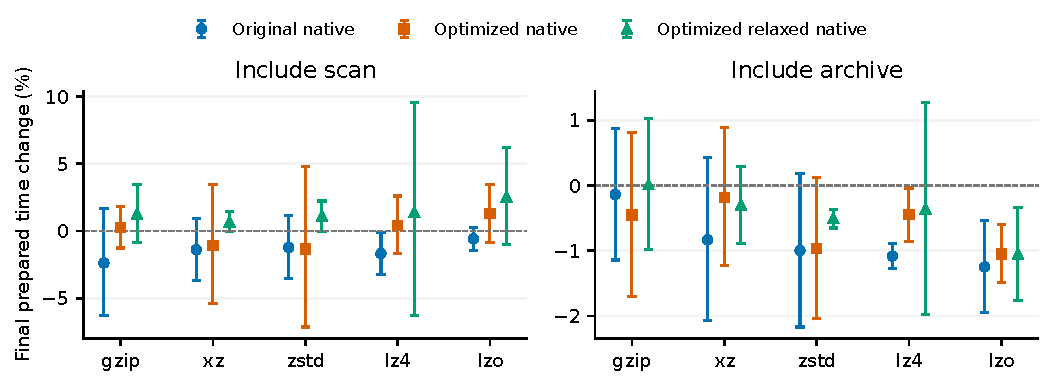
\includegraphics[width=\textwidth]{figures/section65/filesystem-native.pdf}
\caption{Final prepared native versus original, equally optimized normal and
equally optimized relaxed native references. Fresh-mount scan/archive;
pointwise 95\% campaign intervals. Negative values mean lower elapsed time.}
\label{fig:filesystem-native}
\end{figure*}

For the nine nonempty ordinary application tasks, VKSO/copied point estimates range from 0.9901 to 1.0056, with pointwise interval endpoints spanning [0.9584, 1.0255] (Figure~\ref{fig:filesystem-sharing}). Equal-length-path xz/lz4 scan/stream controls have point estimates 0.9608--1.0188 and interval endpoints [0.8435, 1.0945]. The single-CPU gzip-stream change is -0.13\% [-1.02\%, +0.77\%]. The observed interval widths bound the precision of the sharing-cost conclusion; they do not establish universal equivalence.
These comparisons hold the owner instructions, bridge, frontend, cache
policy and translator fixed. Ordinary deployment retains its carrier
paths; the separate xz/lz4 scan/stream diagnostic also equalizes loader-path
lengths. The latter provides the tighter backing control for those four cells.

\begin{figure}[t]\centering
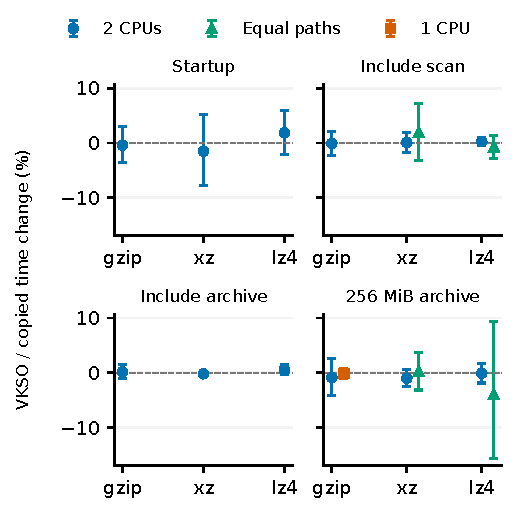
\includegraphics[width=\columnwidth]{figures/section65/filesystem-sharing.pdf}
\caption{VKSO versus identical-core copied execution. All ordinary tasks are
shown; the selected gzip-stream single-CPU check remains a separate condition.
Pointwise 95\% campaign intervals.}
\label{fig:filesystem-sharing}
\end{figure}

\paragraph{Application effects.}
Relative to default SquashFUSE, include-scan elapsed changes range from -54.58\% to -4.42\% and include-archive changes from -19.46\% to -3.30\%. Sequential gzip, xz and lz4 changes are -7.27\% [-10.27\%, -4.17\%], +13.10\% [+11.45\%, +14.78\%], -7.23\% [-11.26\%, -3.02\%], respectively (Figure~\ref{fig:filesystem-application}). Across all twelve ordinary tasks, final VKSO/cache-matched-LKL time ratios range from 0.6323 to 0.9050; the full table retains their per-task intervals.
Against single-thread SquashFUSE, gzip and lz4 include archives instead change by +1.18\% [+0.44\%, +1.93\%] and +0.89\% [+0.65\%, +1.13\%]. The corresponding scans are close in point estimate, whereas xz scan remains faster at -53.59\% [-54.49\%, -52.68\%]. Thus stock threading explains much of the gzip/lz4 metadata advantage over its default configuration, but not the large xz difference.
In a separate xz metadata-work diagnostic, default and single-thread
SquashFUSE each decode 137 blocks and 1,106,363 bytes; the common parser
decodes 76 blocks and 558,231 bytes, whether it uses library or common XZ.
Three replays agree. Reduced decompression work contributes to the metadata
advantage; these counts do not assign the whole time difference to one cause.

\begin{figure*}[t]\centering
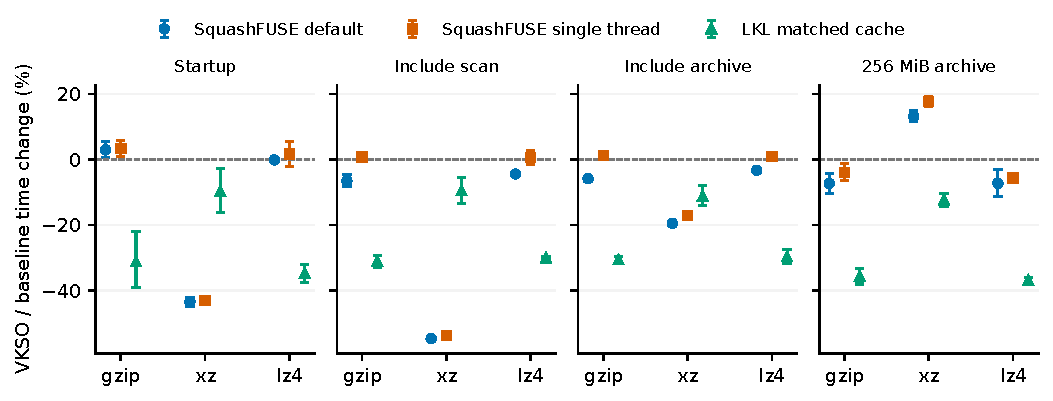
\includegraphics[width=\textwidth]{figures/section65/filesystem-application.pdf}
\caption{Complete VKSO application time relative to default/single-thread
SquashFUSE and cache-matched LKL512. Startup, metadata and sequential tasks
retain their own outcomes and pointwise 95\% intervals.}
\label{fig:filesystem-application}
\end{figure*}

An independent distribution task compiles the Python~3.10 standard library
through real gzip/xz SIFs into a fresh writable bytecode cache. The task and
images were fixed before confirmation and were not used to optimize the
reader. Every backend generates the same 647 bytecode files.
VKSO changes complete compilation time by +0.68\% [+0.22\%, +1.14\%] (gzip) and +16.18\% [+15.56\%, +16.80\%] (xz) relative to default SquashFUSE. Against cache-matched LKL, the changes are -6.05\% [-6.72\%, -5.38\%] and +6.72\% [+6.31\%, +7.13\%], respectively (Figure~\ref{fig:filesystem-heldout}).
This held-out task does not establish a general application speedup: the
additional XZ reuse has a measurable cost, including against LKL for this task.

\begin{figure}[t]\centering
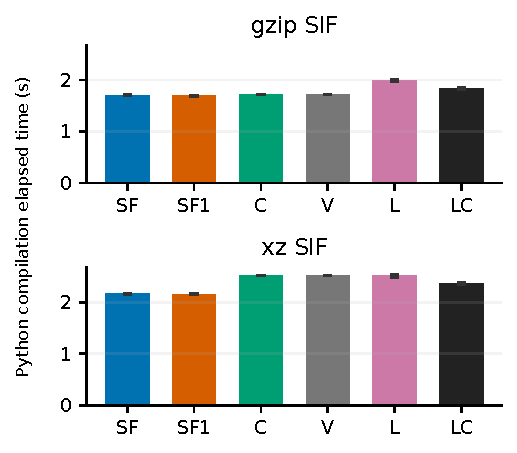
\includegraphics[width=\columnwidth]{figures/section65/filesystem-heldout.pdf}
\caption{Held-out standard-library compilation: mean campaign medians with
pointwise 95\% intervals. SF/SF1: default/single-thread SquashFUSE; C/V:
copied/VKSO; L/LC: default/cache-matched LKL512.}
\label{fig:filesystem-heldout}
\end{figure}

With both external libraries retained, switching from library to common decoding changes xz/lz4 sequential time by +14.79\% [+13.43\%, +16.16\%] / -0.31\% [-2.36\%, +1.78\%]. Removing the now-unused dependencies while retaining common decoding changes it by -0.51\% [-2.45\%, +1.47\%] / +0.89\% [-3.00\%, +4.94\%]. The xz decoder switch changes measured child CPU time by +14.87\%, consistent with an execution-cost difference.
Dependency removal has a small, uncertain effect. The controlled
comparison attributes the final sequential loss primarily to the decoder
execution choice; it does not identify a particular inner-loop cause.
These diagnostics compare library decoding, common decoding with both
libraries retained, and common decoding after dependency removal on the
same owner. They explain final-build tradeoffs without assigning prior
layout-sensitive results to physical sharing.

\paragraph{Engineering and maintenance.}
Reuse preserves the original format/decoder implementations, but requires
explicit preparation and domain support. Sixteen native source/header files
change, largely through extraction and service exposure. Three of the
34 extracted filesystem bodies differ: device-size access, BIO input
handling, and the maintained/bounded-copy helper. Generated kernel support
and contract headers occupy 390 physical lines. The first user integration
contains a 408-line bridge, 154-line POSIX/codec binding and 300-line FUSE
frontend; the application translator adds 96 lines. Generators, reused LZ4
sources, unchanged XZ algorithms and general-exporter fixes are accounted
separately in the artifact. These measures describe maintenance surfaces;
they do not establish reduced developer hours. LKL's SIF integration adds
30 lines to its existing frontend; incremental application adapters are
compared from an existing-platform starting point in both cases.

The known upstream negative-offset repair is reproduced in isolated guests
across old/fixed native, copied and shared paths. The repair changes the
common implementation while preserving the bridge/frontend in that
maintenance experiment. The final composed owner retains the repaired
filesystem source and passes a new guest regression: native/copied/shared
report EIO, user daemons survive, and normal five-format reads, restoration
and unloading pass. A repair requires rebuilding and redeploying the owner;
copied execution receives the same source-maintenance benefit. The shared
XZ hardware breakpoint and the retained ISO9660 replay demonstrate debugging
of common instructions from the user environment.

\paragraph{Resources and deployment.}
After the include archive, VKSO helper PSS is 7.00--7.04~MiB, compared with 14.16--23.95~MiB for default SquashFUSE, 11.64--12.85~MiB for single-thread SquashFUSE, and 82.57--82.85~MiB for cache-matched LKL. In separate untimed metadata-scale runs, VKSO retained PSS is 7.02, 23.43, 88.89~MiB after visiting 5,866, 23,464 and 93,856 entries. At the largest scale, default/single-thread SquashFUSE and cache-matched LKL retain 28.52, 12.91, 500.92~MiB, respectively. The scale result exposes the cost of retaining private metadata; the small-tree footprint is not a fixed runtime-memory bound.
The bridge retains its inode/name lists until unmount and has no eviction
policy. This implementation choice accounts for growth in visited metadata;
the compact-runtime result applies to the small trees, not to all mount sizes.
\begin{table}[t]\centering\small
\caption{Helper PSS after include archive, before PFN observation. Ranges span three codecs and three campaigns; they are not peaks.}
\label{tab:filesystem-resources}
\begin{tabular}{lr}\toprule Backend & PSS range (MiB) \\\midrule
SF & 14.16--23.95 \\
SF1 & 11.64--12.85 \\
C & 6.99--7.04 \\
V & 7.00--7.04 \\
L & 82.53--82.81 \\
LC & 82.57--82.85 \\
\bottomrule\end{tabular}\end{table}

The installed-platform premise treats the generic 32~KiB
\texttt{page\_cache\_replace} module as one-time infrastructure. Filesystem
preparation and per-core registration remain business costs
(Table~\ref{tab:filesystem-business}).
An already prepared native service can avoid one 36~KiB user backing while
requesting 1,264 bytes of registration metadata. Relative to a matched native
module reference, the prepared owner/consumer adds 48~KiB of component residency. User-only
deployment retains the 68~KiB owner; an actual SIF run succeeds without the
native consumer or construction observer, whereas copied execution also
succeeds after all task modules unload. Ordinary copied DSOs share between
user processes, so avoided backing has no process-count multiplier.
\begin{table}[t]\centering\small
\caption{Filesystem component costs with the generic platform installed. Residency, avoided backing and requested metadata are separate quantities.}
\label{tab:filesystem-business}
\begin{tabular}{lr}\toprule Component & Size \\\midrule
Matched native module & 60 KiB \\
Prepared owner + consumer & 108 KiB \\
Native preparation increment & 48 KiB \\
Avoided core backing & 36 KiB \\
Requested registration metadata & 1,264 B \\
\bottomrule\end{tabular}\end{table}

Across nine ordinary application campaigns, core construction, export and registration take a median 2.698~s (observed range [2.696, 6.088]~s), excluding compilation, module loading and validation. This setup is reused by later invocations while the owner and registration remain installed; an owner reload or version change requires fresh deployment. Copied artifact construction also has a setup cost, so these measurements do not assume that its preparation is free.
Module residency, requested allocations and process PSS remain separate
ledgers; the case does not establish whole-machine net-memory savings.

The results support a common resident filesystem/decoder body serving
native and real application consumers with private state and one source
repair point. Complete-backend efficiency and maintenance benefits also
apply to copied execution; VKSO adds native/user physical identity with the
measured incremental cost. Performance conclusions cover these read-only
SIFs and tasks on this host/boot. Five-format functionality, boundary-read
correctness and simultaneous lifetimes do not by themselves establish
five-format application speed, random-I/O performance or concurrent scaling.
